\chapter{Results and summary}
\graphicspath{{Chapter5/Figs/}{Chapter5/Figs/}}

This chapter presents the concrete final results, a concise summary of the project in the form of key aspects of a N/CI and an example architecture, while taking into account the initial goals and objectives.

% 5.1 Ergebnisse: Präsentation des konkreten Endergebnisses. Kompakte Zusammenfassung des Projekts unter Berücksichtigung der anfänglichen Zieldefinition. Wichtig ist dabei, dass man eine kritische Betrachtung der faktischen Resultate vornimmt (Evaluation). Hier ist ein Soll-Ist-Vergleich zur Zielsetzung aus Kapitel 1 mit kritischer Stellungnahme gewünscht. 5.2 Zusammenfassung: Es soll eine Zusammenfassung der Arbeit geschrieben werden und ein Fazit in Bezug auf das Projekt dessen Bedeutung (Relevanz und Nutzen) gezogen werden. Weiterhin soll eine Kritische Betrachtung der eigenen Vorgehensweise erfolgen. Abschließend soll ein Ausblick auf weitere Projektideen, die sich im Rahmen der Arbeit ergeben haben, gegeben werden (Folgeprojekte, Veröffentlichungen, Verwertung). Empfohlener Umfang: ca. 15-20%

\section{Results}
\label{chapter5-results}

This section discusses the final results of the implementation chapter. The author begins by discussing the most important key aspects and insights of a N/CI for the software components of the NIP for IDUN, and then delves deeper into architectural aspects of the technical implementation.

\subsection{Key aspects of a N/CI}
\label{chapter5-key-aspects}

The term N/CI is defined by the three-dimmensionality as described in \autoref{fig:nci-definition-intro}. However, this description does not take into account key aspects, e.g. to achieve general applicability of the production-oriented implementation according to the technological definition. The following subsections discuss some of the technical as well as ethical and privacy aspects of the exemplary built N/CI for IDUN Technologies.

\subsubsection{Stream-based events}
\label{chapter5-stream-based-events}

One of the most important technical aspects of a N/CI is the stream-oriented and even-driven architecture. An event-driven architecture is common in modern applications built with microservices and uses events to trigger and communicate between decoupled services \citep{amazon_web_services_inc_event-driven_nodate}. The stream-oriented aspect describes the main events happening in such a system. Neural data recorded from IDUN's sensors is being streamed from the end-users' devices and processed on the cloud in order to transform and classify the raw data to generate applicable and intelligible output. There are two main differences between the stream types when building a N/CI:

\begin{itemize}
\item \textbf{Synchronous streams} for active and real-time BCI.
\item \textbf{Asynchronous streams} for passive, reactive BCI.
\end{itemize}

Either a user streams neural data from the device to obtain real-time output, such as controlling an object in a game, or to improve audio amplification based on where the user is looking. Such use cases necessitate real-time classification within an acceptable latency (more on latency in the next subsection). Parallel processing of neural data streams is critical, and timestamp synchronisation between different transformed or classified output streams must be prioritised.

The other component occurs when an asynchronous stream is used in place of a real-time stream. For example, while sleeping, the user does not require real-time insights into his sleep. When he awakens, the system must stop the stream, classify it, and display the stages of sleep, for example. These various aspects are significant because some classifications, such as band performance, require a specific time window (epoch) to calculate an understandable output. To determine the proportion of, say, alpha waves (which typically have frequencies between 8 and 13 Hz) in a user's neural data, we must transform it with a fast Fourier transform (FFT), which requires a specific portion of the neural data's time range, i.e. a specific length of epoch. 

\begin{figure}[!ht]
  \centering
  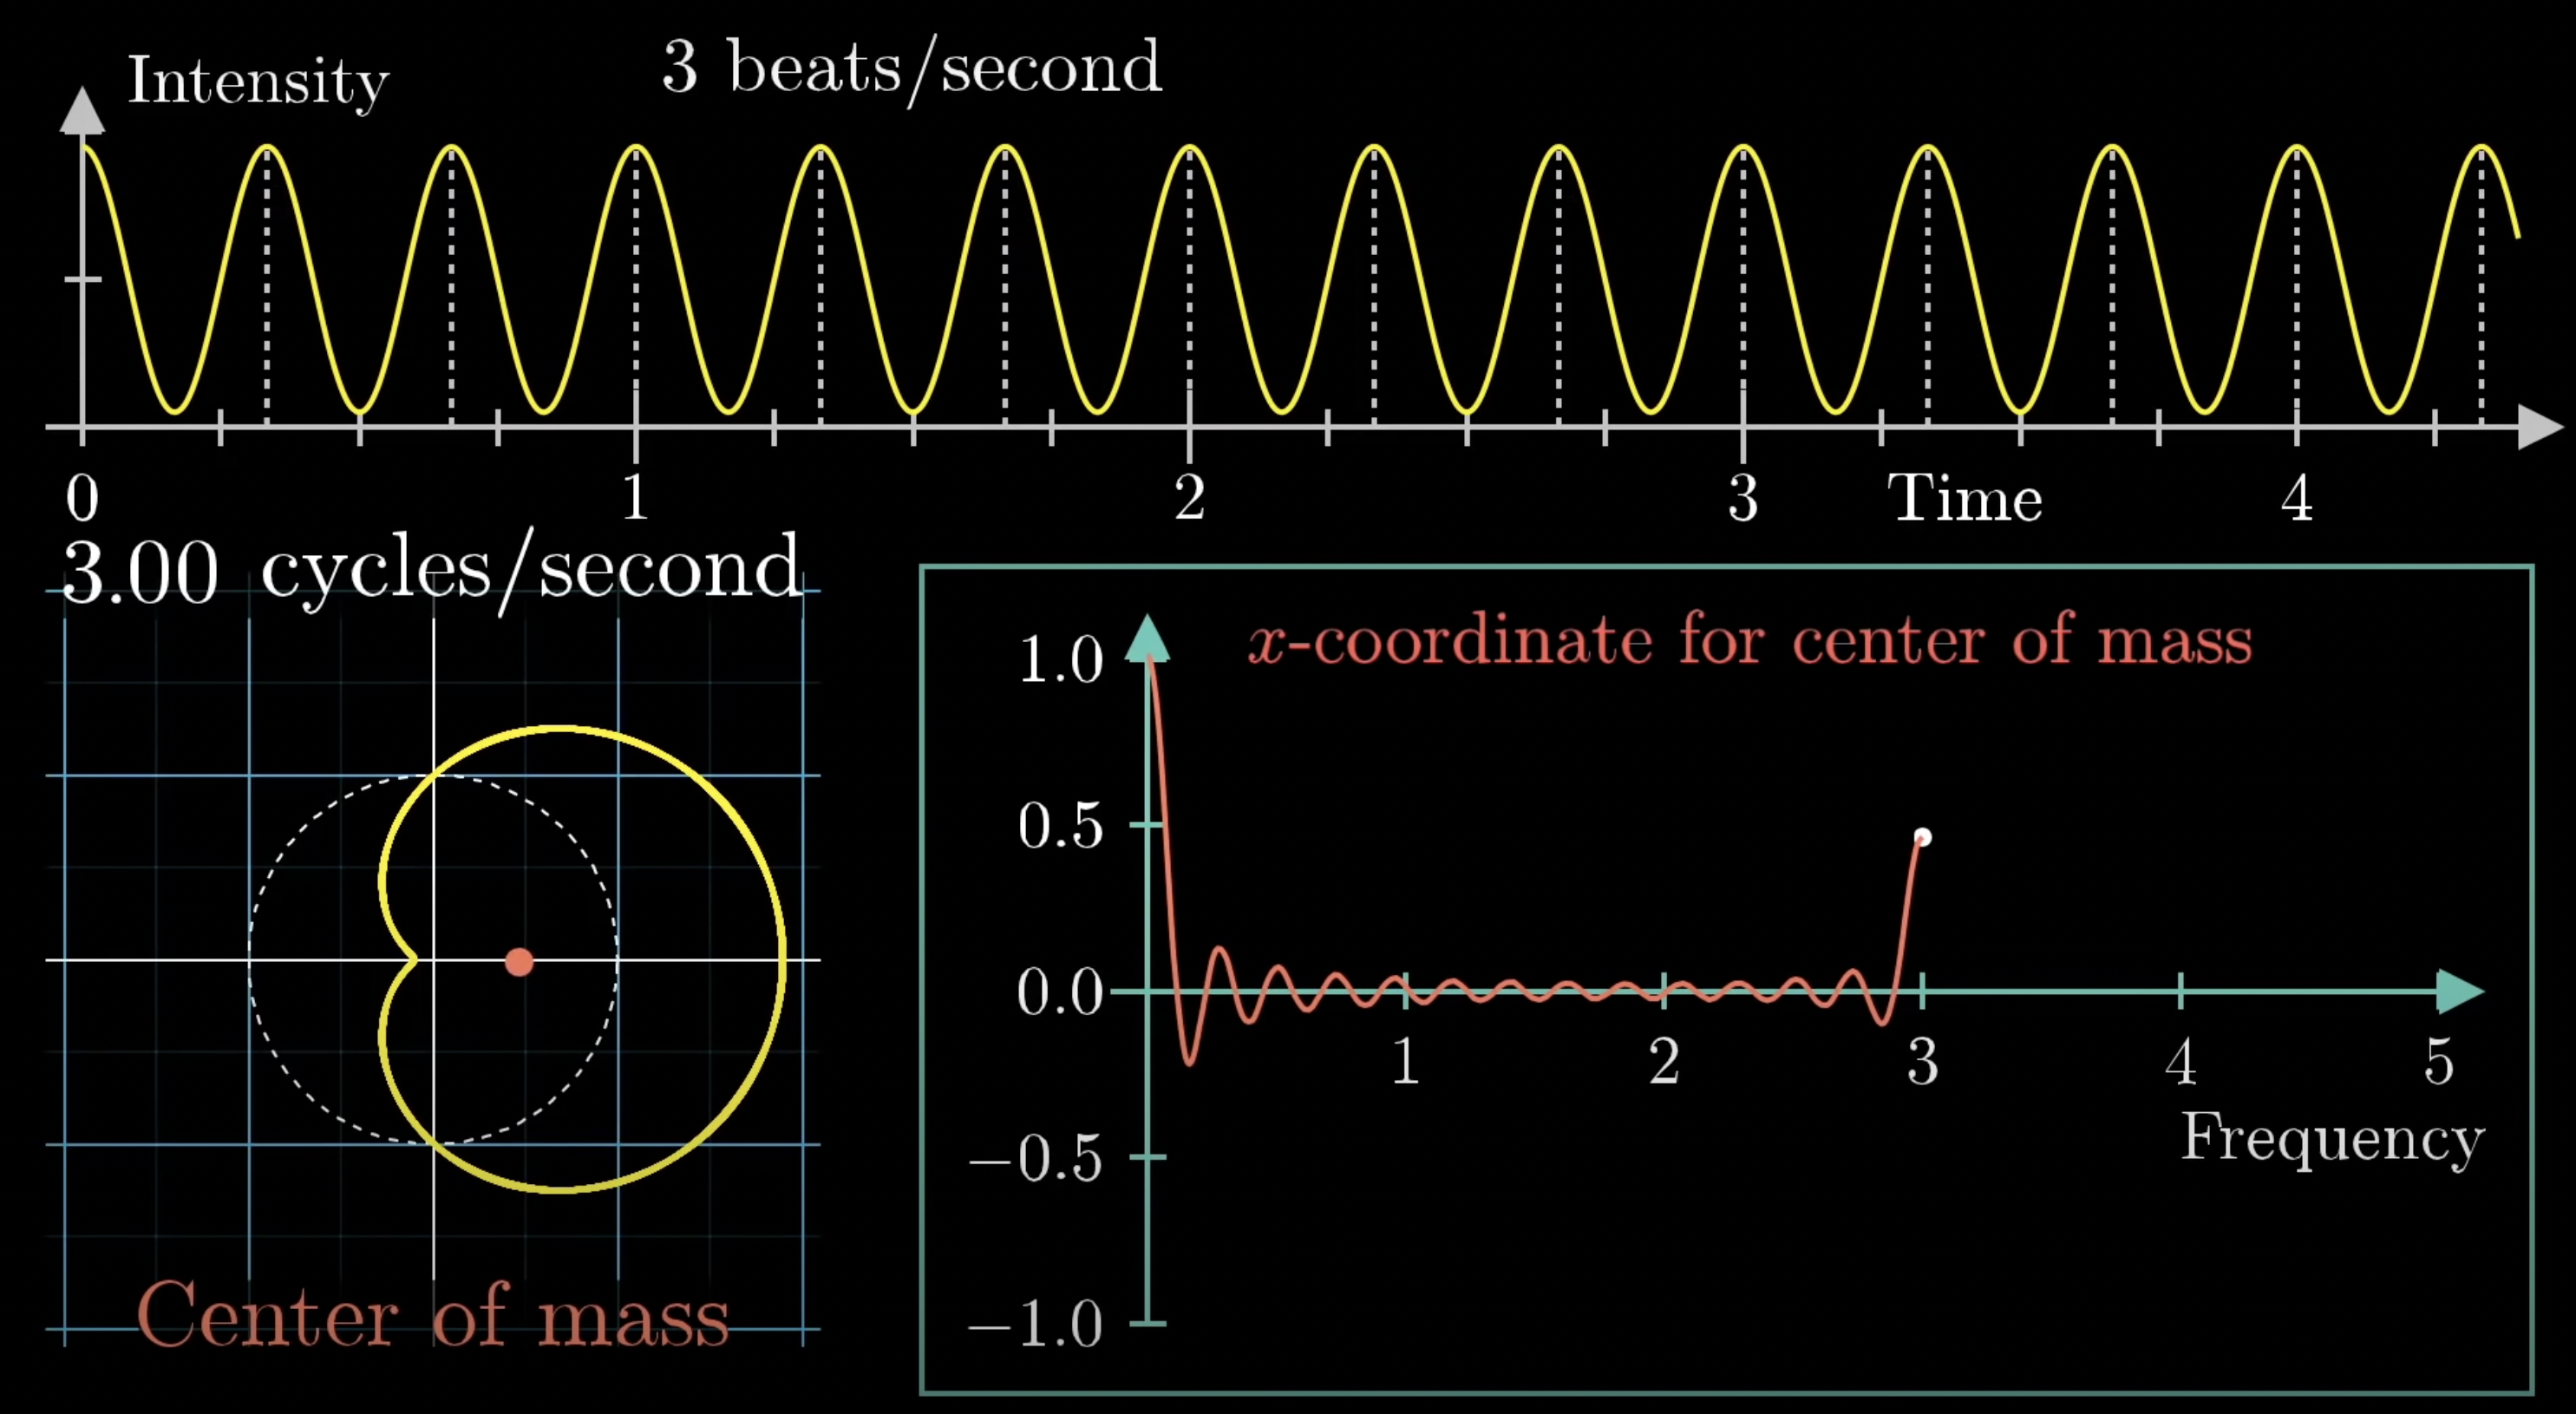
\includegraphics[width=\linewidth]{fft.png}
  \caption[Illustration of how FFT works]{Illustration of how FFT works \citep{3blue1brown_but_2018}}
  \label{fig:fft}
\end{figure}

The process of FFT is represented visually in \autoref{fig:fft} a given frequency in the time series is used to calculate the cycles to extract the originally occurring frequency signal based on the epoch length. As a result, we have per-sample and epoch-based classification of neural data, which can be real-time, real-time with an initial delay to buffer a given epoch (as with FFT), or asynchronous and not real-time, as with sleep phases.

% TODO create figure for epoch vs per sample incl buffering

\subsubsection{Critical and non-critical}
\label{chapter5-critical-and-non-critical}

The topic of stream-based events brings up the issue of critical and non-critical use cases. A synchronous neural stream with low-latency classification of whether the driver is currently awake, asleep, or about to fall asleep is required in a critical use case such as microsleep detection while driving. In such cases, the classification must be as fast as possible, as in per-sample classification or epoch-based classification (most likely with buffer), so the connection speed between the measurement sensor and the classifier is more important. In extremely critical use cases, where a user's life may depend on it, the classification would need to be done without an active internet connection, so that the classification model runs on the hardware itself rather than in the cloud, in order to intervene within milliseconds (e.g., in the form of a loud sound to warn or wake up the driver), as a few moments can mean the difference between fatalities.

Not-so-critical applications can fall back on non-offline modes and run classifiers over an active internet connection in the cloud. To reduce latency, edge cloud computing could be introduced, where business logic executed in the cloud is brought geographically closer to the end user via edge locations \citep{nomios_what_nodate}.

The distinction between critical and non-critical streams can be made not only for synchronous streams, as described in the preceding examples, but also for asynchronous streams, particularly in the context of research. In general, research like that represented by IDUN's Persona Noel does not necessitate synchronous streams or classifications, but rather the most reliable possible acquisition of neural data from test subjects. The critical aspect in such a use case can also be much higher than, for example, recording neural data during sleep in consumer-oriented applications. For example, if the device goes offline or the Bluetooth connection is lost, the device must cache the data locally and be able to restore it once the device is back in range or a sufficiently stable internet connection is restored. The author recommends having a fallback system in the form of buffering for each data stream, for example, if neural data becomes corrupted or misordered due to timestamp mismatches in the cloud.

% TODO create figure for buffering on device and on phone when offline or out of range

\subsubsection{Encryption and opt-in}
\label{chapter5-user-side-opt-in}

Because IDUN develops an unobtrusive library (in the form of an SDK, as detailed in \autoref{appendix4-further-key-events}) that can be easily implemented in existing software such as web apps or mobile apps, the developers of these apps have actual access to the hardware and initiate the Bluetooth connection between the sensor and the end-user device. IDUN must encrypt the recorded data on the hardware before it reaches the third-party app to protect user privacy and the security of end-user neural data. This is a critical step in preventing third-party providers from collecting extensive data and classifying insights from users that they may not want. In the asynchronous encryption example, IDUN securely decrypts the data in its cloud using the private key.

% TODO show figure of how encryption works with private keys etc.

Third-party developers can thus only access data that the user has authorised. The duration of data storage, the type and level of detail of certain classifications of their neural data, and sharing and usage analysis are all opt-in options. Figure 3 depicts how such an opt-in mechanism might appear as a GUI in a third-party mobile app.

% TODO show opt-in mechanism (say that the full version is in the appendix 123)

The fact that unencrypted raw data should never be accessible to third parties poses some technical challenges. To visualise and display the raw time series of IDUN's EEG sensors, for example, the individual display images would have to be rendered on the server side and streamed to the client as video. Another difficulty is synchronising and organising the rotation of public and private keys, which must be done without interference from third parties. Envelope encryption, as shown in Figure 3, is a tried and true method for this \citep{google_cloud_envelope_nodate}.

% Show figure of envelope encryption \citep{google_cloud_key_nodate}

\subsubsection{Graph data access}
\label{chapter5-graph-data-access}
% explain MLOps and outlook with Kubeflow
% mention data lakes and data warehouse
% mention internal SDK for feature extraction and experiments
% what is feature extraction and the process
% show image from Wadda

% However, in practice, it appears that simply making data available quickly—even if it is in a quirky, difficult-to-use, raw format—is often more valuable than trying to decide on the ideal data model up front [54].

\subsection{Example architecture of a N/CI}
\label{chapter5-example-architecture-of-a-nci}

% split by key components
% show what i've drawn on the whiteboard at work for event-driven architecture

% Performance
% Scalability
% Reliability
% Security
% Deployment
% Technology Stack

% TODO show entire architecture chart and split into sections and go through them figure by figure

% - First, we investigated whether X (research question)
% - We used an Independent samples t test with groups as independent variable and the
% depression score as dependent variable
% - The results showed that the difference between the groups/ conditions was significant
% - The results showed a significant correlation between…
% - The results showed a significant interaction between…
% - Specifically, the average depressions score was lower in the treatment group (M=3.45, SD = 2.18) compared to the placebo group (M=4.83, SD = 2.02).

% Always show measure of success per each part of the architecture (say that going into detail of performance indicators and security is not part of this thesis)
% talk about achieved goals

% o Did you describe everything that is needed to replicate your results?
% o Did you describe all pre-processing steps before the main analyses?
% o Did you mention to which research question each analysis belongs?
% o Did you avoid interpreting your results?
% o Did you add figures for making your key results easy to understand (or are they very simple)?
% o Did you add tables for extensive amounts of (numerical) information?

% o Does your discussion go from specific (interpretation) to broad (implications)?
% o Did you draw conclusions with reservations? (“A possible interpretation is…”)
% o If you expressed a preference for one explanation over another, did provide clear
% support for this preference?
% o Did you describe how your research connects to previous research?
% o Did you make clear what your research adds to existing research?
% o Did you describe how your research advance our understanding or how they may inspire
% future applications?
% o Did you clearly admit limitations before qualifying them?
% o Did you remind the reader of the value/implications of your research at the end?
% o Did you include some pointers for future research? (optional)

% non-trivial, n-body system, Services, batch processing and near real time streaming, shared nothing, encrypted, total order broadcast etc. => all insights that were gained for the N/CI and the task to define a N/CI on its own as well + Systems of record and derived data system (p 602 to cite) ==> add some parts to the implementation chapter

\section{Summary}
\label{chapter5-summary}

\subsection{Reflection}
\label{chapter5-reflection}

\subsection{Outlook}
\label{chapter5-outlook}
% mention to publish the thesis somewhere if possible with the help of IDUN
% further development into deep learning models and more detailed description of a N/CI on the cloud rather then "just" introducing and displaying the most important aspects and components => could be done in a MSc

\subsection{Conclusion}
\label{chapter5-conclusion}

% - We investigated whether depression can be treated by training a positive focus
% - Our findings confirm this
% - Novel perspective on depression
% - More research needed, more treatments that follow this approach should be developed

\nomenclature[fft]{fft}{Fast Fourier transform}